\chapter{RNA Base Pair Steps}
\label{basepairsteps} 
\bibliographystyle{nar} 
Before  the turn  of the  century it  was still  not  conceivable that
knowledge-based potentials  could be obtained for  RNA helical regions
due to the  small amount of crystallographic data  available. This was
not the case for DNA, where  enough data for such potentials have been
available   since   1998  as   shown   by   Olson  and   collaborators
\cite{olson1998}.   As  pointed  out  in  Chapter  2,  the  number  of
high-resolution X-ray  crystal structures of RNA has  increased by two
orders of magnitude, giving us enough information to develop a dimeric
model of double-helical  RNA with 10 unique base-pair  steps formed by
the canonical G$\cdot$C and  A$\cdot$U Watson-Crick pairs. An extended
model with 21  unique dimeric steps can also  be constructed by adding
the wobble G$\cdot$U base-pair  to canonical G$\cdot$C, and A$\cdot$U,
but GU$\cdot$GU (11 cases) and UA$\cdot$UG (20 cases) dimeric data are
still  scarce. An illustration  of the  possible unique  dimeric steps
which can be formed in RNA is given in Figure \ref{fig:unique}.

\begin{figure}
\centering
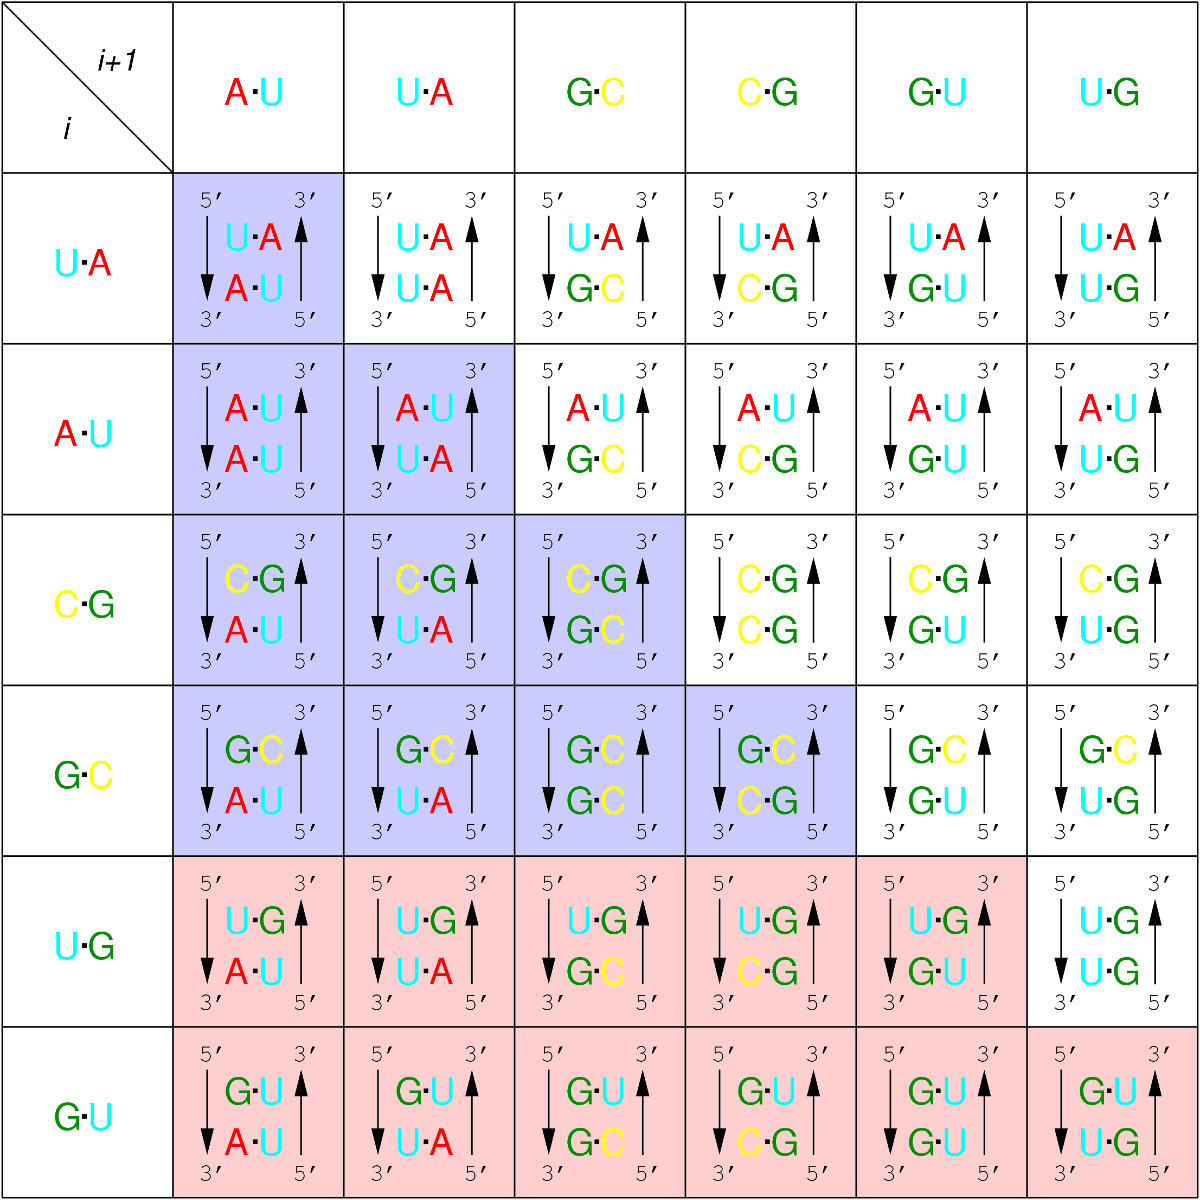
\includegraphics[angle=0, scale=0.4]{Chapter4/unique.png}
\caption{Color-coded representation of  the 21 unique base-pair dimers
of RNA  formed by canonical G$\cdot$C, and  A$\cdot$U Watson-Crick and
wobble  G$\cdot$U base-pairs.  The  grey boxes  include the  10 unique
base-pair steps  formed by canonical G$\cdot$C and  A$\cdot$U, and the
pink  boxes  the  additional  11  base-pair steps  which  result  from
considering G$\cdot$U wobble base-pairs  as dimer building blocks. The
coloring scheme  used to  denote the  bases is that  used in  the NDB,
where A  is red, U is  cyan, G is green,  and C is  yellow.  The first
base-pair X in  each XpY step in the 5$'$ to  3$'$ sense is identified
as pair $i$ and the second Y  is identified by $i+1$ in the upper left
corner of the figure.}
\label{fig:unique}
\end{figure}  

For the case  of the 91 possible unique base-pair  steps, which can be
formed from the seven dominant base-pairing types discussed in Chapter
3, we see  tendencies of favored sequences infered  from counts of the
available data as will be shown in the next section.

The results obtained from  the analysis of RNA knowledge-based dimeric
information  allow us  to  explore double-helical  RNA  at the  global
level,  that is,  as a  polymer chain.  Therefore we  can  compute the
persistence length of some RNA  sequences as shown in the last section
of this chapter.

\section{Base-Pair-Steps in Intact Helical Regions} 
From  the  dataset  of  base-pairs  described in  Chapter  2  we  also
collected base pair step information  and focused our attention on the
dimers which are  located in intact helical regions,  those noted as H
in  Figure   \ref{fig:helregxin}.   From  the  data   shown  in  Table
\ref{tab:91steps} we  see that it  is more common for  a non-canonical
base-pair to abut a canonical base-pair than a non-canonical one.  The
number of  steps formed by  a non-canonical base-pair and  a canonical
one  is  six   times  greater  than  that  of   steps  formed  by  two
non-canonical  pairs.  A few  non-canonical  base-pairs  occur in  the
context     of    a    stack     of    non-canonicals,     e.g.,    13
GA$_{\text{s}}$$\cdot$GA$_{\text{s}}$              and              20
GA$_{\text{s}}\cdot$A$_{\text{s}}$G    steps,   where    two   sheared
base-pairs stack  together, and 32 AG$_{\text{s}}\cdot$GU$_{\text{w}}$
where  a sheared  G$\cdot$A$_{\text{s}}$  base pair  stack  next to  a
Hoogsteen         A$\cdot$U$_{\text{H}}$         base-pair,         42
GU$_{\text{w}}\cdot$GU$_{\text{w}}$              steps,             31
UG$_{\text{w}}\cdot$GU$_{\text{w}}$               and               11
GU$_{\text{w}}\cdot$U$_{\text{w}}$G.   The majority of  stacks between
non-canonical   base-pairs  occurs  on   dimeric  steps   composed  of
combinations  of G$\cdot$U  wobble and  sheared  G$\cdot$A base-pairs.
Overall the majority of dimeric steps ($(604+608+1335)/6755 = 37.7\%$)
are those formed by canonical G$\cdot$C base-pairs making up more than
a    third   of   the    whole.    Furthermore,    GG$\cdot$CC   steps
($1335/(604+608+1335) = 52.4\%$) form more  than half of these kind of
steps.

Overlap values between base-pairs  are given in parentheses along with
the  counts  of dimeric  steps  in  intact  helical regions  in  Table
\ref{tab:91steps}. Examination  of these values shows  that the common
trends  seen for  overlaps of  DNA  base-pairs persist  in RNA,  i.e.,
purine-pyrimidine  (RY) steps  have the  greatest overlap  values, and
pyrimidine-purine  (YR)  the  smallest.   When  the  G$\cdot$U  wobble
base-pair is taken into consideration  the trend remains true, but the
values   are   considerably    increased,   for   example,   for   the
GU$_{\text{w}}\cdot$UG$_{\text{w}}$  dimer the  overlap value  is 14.4
\AA$^{\text{2}}$    compared     to    11.3    \AA$^{\text{2}}$    for
GC$_{\text{WC}}\cdot$CG$_{\text{WC}}$. Other dimers which show a large
overlap include those composed  of sheared G$\cdot$A pairs and sheared
G$\cdot$A and  U$\cdot$U wobble pairs.  The degree  of overlap doesn't
necesarily correlate with greater dimer stabilities as judged from the
populations of observed  dimers. For example, there are  more cases of
wobble U$\cdot$U  pairs adjacent to canonical G$\cdot$C  pairs than to
canonical A$\cdot$U pairs despite the smaller overlap area.

\begin{sidewaystable}
%\begin{table}[hb]  
\begin{center}
%\scalebox{0.7}{
\begin{tabular}{|c|c|c|c|c|c|c|c|c|c|c|c|c|c|c|}
\hline
C$\cdot$G$_{\text{WC}}$ & G$\cdot$C$_{\text{WC}}$ & U$\cdot$A$_{\text{WC}}$ &
A$\cdot$U$_{\text{WC}}$ & U$\cdot$G$_{\text{w}}$ &
G$\cdot$U$_{\text{w}}$ & A$\cdot$G$_{\text{s}}$ &
G$\cdot$A$_{\text{s}}$ & U$\cdot$A$_{\text{H}}$ &
A$\cdot$U$_{\text{H}}$ & U$\cdot$U$_{\text{w}}$ &
A$\cdot$G$_{\text{WC}}$ & G$\cdot$A$_{\text{WC}}$ & bp$_{i}$/bp$_{i+1}$\\ 
\hline  
604$_{(\text{4.5})}$ & 1335$_{(\text{4.1})}$ & 747$_{(\text{3.0})}$ & 574$_{(\text{2.9})}$ & 77$_{(\text{5.0})}$ & 192$_{(\text{5.3})}$ & 66$_{(\text{6.9})}$ & -- & -- & -- & 18$_{(\text{2.9})}$ & 4$_{(\text{4.8})}$ & 5$_{(\text{4.2})}$ & G$\cdot$C$_{\text{WC}}$\\
 & 608$_{(\text{11.3})}$ & 511$_{(\text{4.1})}$ & 572$_{(\text{9.9})}$ & 161$_{(\text{2.9})}$ & 252$_{(\text{13.5})}$ & 33$_{(\text{10.0})}$ & -- & -- & -- & 69$_{(\text{6.1})}$ & 20$_{(\text{8.8})}$ & 5$_{(\text{7.7})}$ & C$\cdot$G$_{\text{WC}}$\\
 &  & 97$_{(\text{2.0})}$ & 249$_{(\text{3.3})}$ & 20$_{(\text{2.8})}$ & 45$_{(\text{6.1})}$ & 7$_{(\text{7.7})}$ & -- & -- & -- & 2$_{(\text{3.6})}$ & -- & 3$_{(\text{4.3})}$ & A$\cdot$U$_{\text{WC}}$\\
 &  &  & 126$_{(\text{8.4})}$ & 48$_{(\text{2.0})}$ & 79$_{(\text{11.8})}$ & 6$_{(\text{9.5})}$ & -- & -- & -- & 20$_{(\text{8.2})}$ & 1$_{(\text{6.4})}$ & 14$_{(\text{5.3})}$ & U$\cdot$A$_{\text{WC}}$\\
 &  &  &  & 31$_{(\text5.3{})}$ & 42$_{(\text{4.1})}$ & 32$_{(\text{8.3})}$ & 1$_{(\text{5.7})}$ & -- & -- & 5$_{(\text{2.9})}$ & -- & -- & G$\cdot$U$_{\text{w}}$\\
 &  &  &  &  & 11$_{(\text{14.4})}$ & -- & -- & -- & -- & -- & 4$_{(\text{8.8})}$ & 7$_{(\text{9.3})}$ & U$\cdot$G$_{\text{w}}$\\
 &  &  &  &  &  & -- & 13$_{(\text{10.6})}$ & -- & -- & 6$_{(\text{11.1})}$ & -- & -- & G$\cdot$A$_{\text{s}}$\\ 
 &  &  &  &  &  &  & 20$_{(\text{9.1})}$ & 7$_{(\text{3.0})}$ & 2$_{(\text{3.7})}$ & -- & -- & -- & A$\cdot$G$_{\text{s}}$\\
 &  &  &  &  &  &  &  & -- & -- & -- & -- & -- & A$\cdot$U$_{\text{H}}$\\
 &  &  &  &  &  &  &  &  & -- & -- & -- & -- & U$\cdot$A$_{\text{H}}$\\
 &  &  &  &  &  &  &  &  &  & 3$_{(\text{1.7})}$ & -- & -- & U$\cdot$U$_{\text{w}}$\\
 &  &  &  &  &  &  &  &  &  &  & -- & 1$_{(\text{6.3})}$ & G$\cdot$A$_{\text{WC}}$\\
 &  &  &  &  &  &  &  &  &  &  &  & -- & A$\cdot$G$_{\text{WC}}$\\
\hline
\end{tabular}
%}
\caption{Counts   of  unique   base-pair  steps   and   overlap  areas
(subscripted  values  in parenthesis)  values  in  intact RNA  helical
regions of RNA structures.}
\label{tab:91steps}
\end{center}
%\end{table}
\end{sidewaystable}


%Using information derived from a 3.5 Å parsed subset of the
%BPS (Base Pair Structure) database [2] and so-called “inverse harmonic
%analysis” [3], we have derived elastic force constants for the 21
%unique base-pair steps, and are using this simple scoring potential
%model to simulate the fluctuations of RNA helical structures.

\section{RNA Base-Pair-Steps Database and Webframework}
With  the  step-parameters from  the  intact  helical  regions we  can
construct  a harmonic  energy function  model. That  is, we  can treat
succesive  base-pairs  as  rigid  blocks  connected by  a  spring  and
described by a harmonic potential function $\Psi(x)$:
\begin{gather}
\Psi (x) = \frac{1}{2}\sum_{i,j} F_{i,j} \Delta x_{i} \Delta x_{j}\\
\Delta x_{i}=x_{i}-x_{i}^{0}
\end{gather} 
Here the  $x_{i}$ represent the spatial arrangements  of the base-pair
steps in terms  of the six rigid-body base  pair step parameters, that
is, the displacements  in Shift, Slide and Rise,  and the rotations in
Tilt, Roll,  and Twist. It has  been shown by Go  and Go \cite{go1976}
that the  correlation of  spatial variables can  be obtained  from the
force constants $F_{i,j}$. That  is, they show that these correlations
are proportional  to $kT$ with a proportionality  coefficient equal to
the $i,j$  elements of the  inverse matrix of second  derivatives with
respect to energy, i.e., the $F$ matrix,
\begin{gather}
\left<x_i x_j\right> = kT (F_{n}^{-1})_{i,j}
\end{gather} 
where  $\left< x_i  x_j \right>$  stands for  the  correlation between
base-pair-step parameters displacements,  $k$ is  Boltzman's constant,
and $T$ is  temperature, an analog to the  ``classical'' treatment for
atoms  by Wilson  et al.  \cite{wilson1955}. By  contrast we  take and
inverse  approach   and  extract  the  $F_{i,j}$   from  the  observed
correlation of variables.

The total potential for a system  of $N$ base-pair steps would then be
given by:
\begin{gather}
U(x_{i}) = \sum_{n=1}^{N} \Psi_{n}
\end{gather}

In order to obtain  quasi-Gaussian distributions of the base-pair step
parameters and  also to exclude extreme  conformational deformation in
steps, we  culled our data by  restricting it to be  within 3 standard
deviations from  the mean  value of step  parameters. These  data were
then  used  to obtain  the  force  constants  by finding  the  inverse
correlation matrix.

A  minimal MySQL database  was created  to store  the mean  values and
covariance  of base-pair-step  parameters, their  standard deviations,
the  derived force-constant  matrices, and  step  deformation measures
such  as  the  conformational  volume,  and the  RMSD  for  all  atoms
excluding hydrogen from the average structure. The purpose of creating
the  database is  for  ease of  sharing  information with  force-field
developers and future automatization of the process of data reduction.
The process of data reduction can be summarized as follows:
\begin{itemize}
\item{Collection   of   a   non-redundant   dataset   of   RNA   X-ray
crystallographic  structures  restricted  to resolutions  better  than
3.5~\AA ~with up-to-date data from the PDB.}
\item{Computation of  base-pair and base pair step  parameters for all
    structures using 3DNA \cite{lu2003}.}
\item{Determination   of   the   Leontis-Westhof   classification   of
base-pairs using rnaview \cite{yang2003}.}
\item{Construction   of  a   relational  database   to   link  various
classifications  of   RNA  structure,  such   as  the  Leontis-Westhof
classification of  base pairs to  the helical classification  given by
3DNA.}
\item{Selection of steps present in intact helical regions alone.}
\item{Culling    unique   base-pair    step    parameters   using    a
    three-standard-deviation cutoff.}
\item{Computation  of the  means, standard  deviations, force-constant
matrices, and other step-deformation measures.}
\end{itemize}  

The    database   and    its   web-framework    can   be    found   at
\url{http://rnasteps.rutgers.edu/}.  The site  includes the  table for
the  21  unique dimers  formed  by  canonical Watson-Crick  G$\cdot$C,
A$\cdot$U, and wobble G$\cdot$U, shown in Figure ~\ref{fig:average}.

\begin{figure}[htbp]
\centering
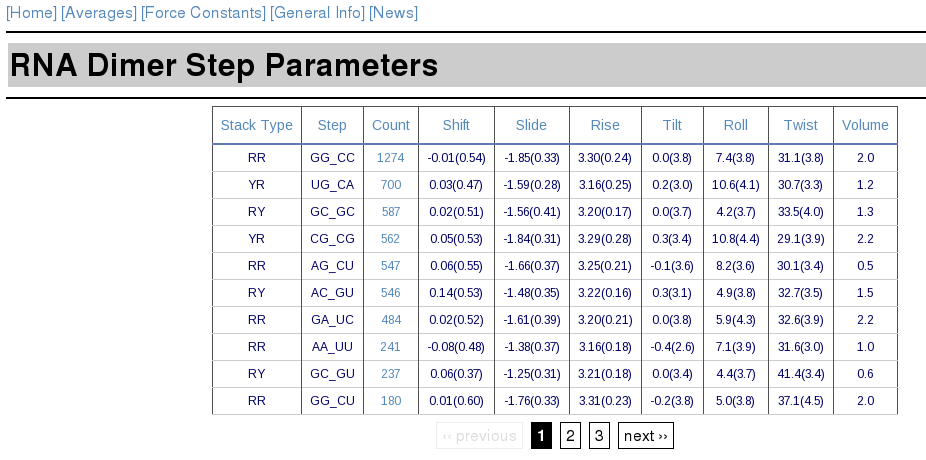
\includegraphics[angle=0, scale=0.5]{Chapter4/average.png}
\caption{Snapshot of  the unique  base-pair step parameters  table for
intact helical  regions of RNA, showing  the fields by  which the data
can  be  sorted. In  this  case  the data  are  sorted  by dimer  step
counts.   There   are    three   stack   types   purine-purine   (RR),
pyrimidine-purine  (YR),  and purine-pyrimidine  (RY).  The steps  are
denoted in a  5$'$ to 3$'$ sense, e.g., GG\_CC  stands for a G$\cdot$C
base-pair  step  covalently linked  between  the  G's  in the  leading
strand,  i.e., GpG,  and the  C's in  the complementary  strand, i.e.,
CpC.}
\label{fig:average}
\end{figure}  

The values in  the table can be sorted by any  of the included fields,
that  is, Stack  Type, Step  Count,  Shift, Slide,  Rise, Tilt,  Roll,
Twist, Volume,  and RMSD. Also  the scatterplot corresponding  to each
step is  displayed when  the users click  on the counts  column, along
with a  potential energy contour in  the Roll-Twist plane  at 4.5 $kT$
(i.e.  3 standard deviations).   A snapshot  of the  roll-twist energy
contour for  the GG$\cdot$CC step  from the web-framework is  shown in
Figure  ~\ref{fig:contour} Note  the lack  of correlation  between the
variables  compared to  the  same steps  in  in DNA  and the  slightly
greater variation in roll compared to twist.
\begin{figure}[htbp]
\centering
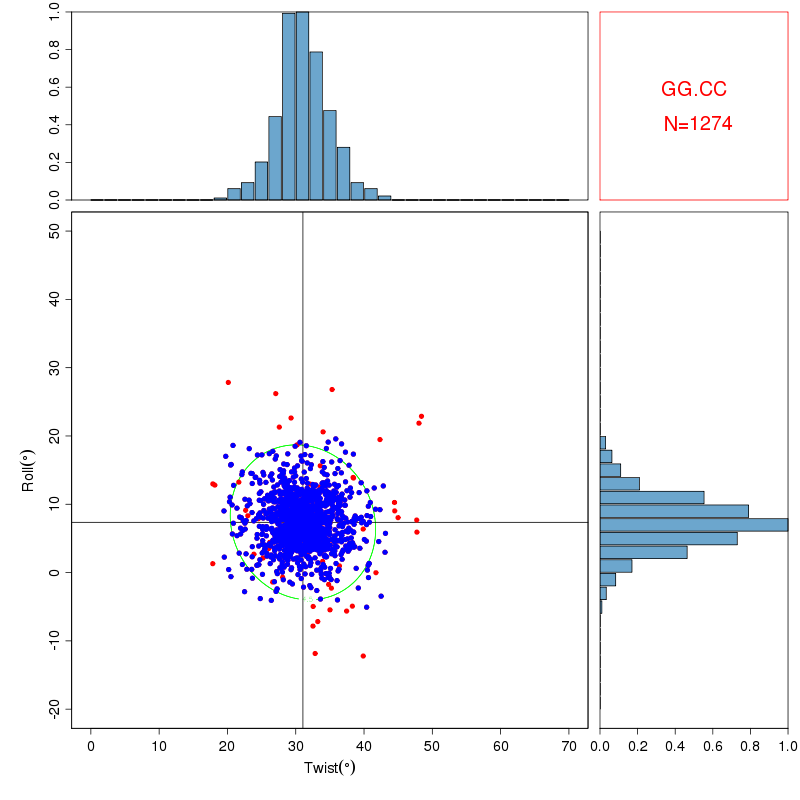
\includegraphics[angle=0, scale=0.54]{Chapter4/contour.png}
\caption{Snapshot  from  the web-framework  of  a  scatterplot in  the
  Roll-Twist plane  with an energy  contour at 4.5$kT$. The  full data
  before culling are depicted in red dots, and the culled data, within
  3 standard deviations of the mean, by blue dots.}
\label{fig:contour}
\end{figure}

The other values included in the web-framework are the force-constants
corresponding to  the unique steps.  A snapshot of  the force-constant
matrix    for   the    GG$\cdot$CC   step    is   shown    in   Figure
~\ref{fig:forceconst}

\begin{figure}[htbp]
\centering
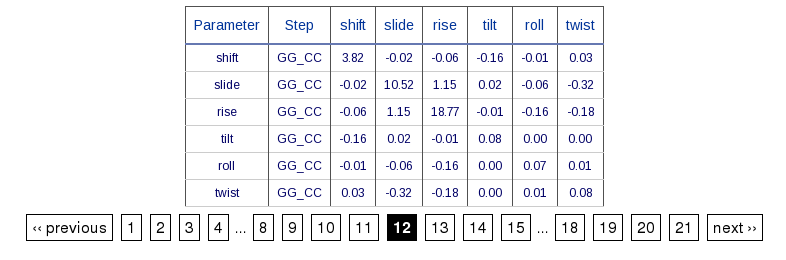
\includegraphics[angle=0, scale=0.6]{Chapter4/forceconst.png}
\caption{Snapshot of  the RNA base-pair-steps  web-framework where the
  force constant matrix for the GG$\cdot$CC dimeric step is shown. The
  force  constant  matrix  is  derived  from the  covariance  of  step
  parameter  values following  Go and  Go \cite{go1976}  and  Olson et
  al. \cite{olson1998}.}
\label{fig:forceconst}
\end{figure}  

\section{Persistence Length of RNA}
A quantity commonly used to  quantify the stiffness of polymers is the
so-called persistence  length $a$. To determine this  quantity for DNA
or RNA,  a variety of  theoretical and experimental techniques  can be
used.  Some  common experimental  techniques to determine  $a$ include
electron   microscopy   (EM),   gel   electrophoresis,   sedimentation
velocities, electrical birefringence,  atomic force microscopy (AFM) ,
magnetic  tweezers,  and small  angle  X-Ray  scattering (SAXS).   For
reviews  of  such  techniques  applied  to the  determination  of  RNA
persistence    length,    we   refer    the    reader   to    Hagerman
\cite{hagerman1997}, Abels  et al.  \cite{abels2005},  and Caliskan et
al.  \cite{caliskan2005}.  We compare  our simulated results, based on
the observed  structural properties of  RNA and the  "realistic" model
developed by Olson and collaborators \cite{marky1994a, maroun1988a} to
describe  DNA,  with the  persistence  length  extracted from  various
experimental means.

Initial studies started with  selected data for the deformabilities of
the  ten unique  base-pair  steps \cite{olson1995}.   A more  complete
picture applied  to the study of  DNA sequence-dependent deformability
became  available   in  1998  \cite{olson1998}.    The  base-pair-step
deformability  data  for  DNA  have  been constantly  refined  as  more
high-resolution DNA and DNA-protein  structures have been added to the
Nucleic Acid Database (NDB) \cite{balasubramanian2009}.  Although such
data have been available for DNA  since 1998, such was not the case for
RNA, until recently \cite{olson2009}.

A brief description of the ``realistic'' model along with a simplified
schema  of the  C++ code  developed by  Dr. Luke  Czapla  and modified
slightly by  the author,  is given in  Appendix~\ref{appendix4a}. This
Appendix  also includes  a brief  account of  various  definitions and
models generally used to compute persistence length in the literature.


\begin{figure}
\centering
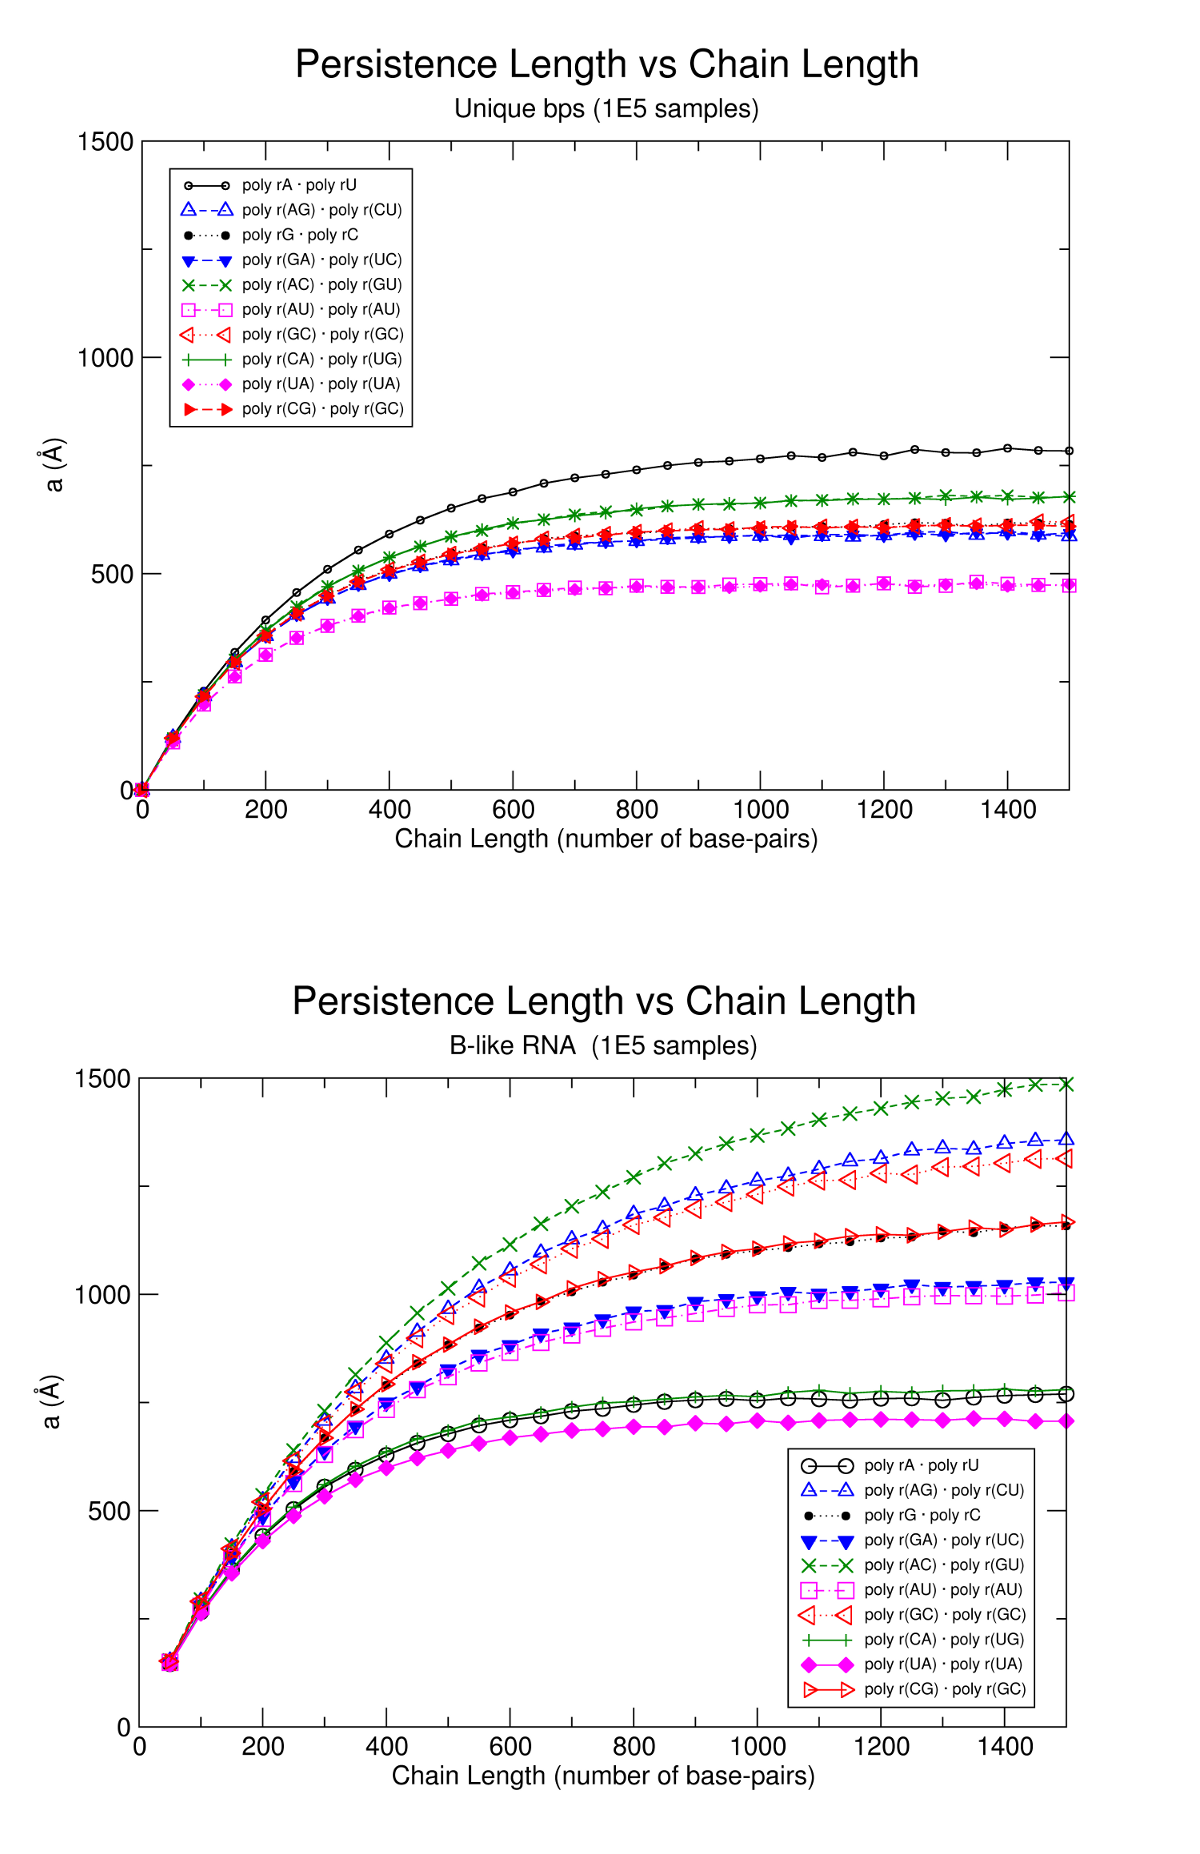
\includegraphics[angle=0, scale=2.6]{Chapter4/perVlen.png}
\caption{In  the lower  frame persistence  length vs  chain  length in
  base-pairs  for naturally  straigth chains  with 11  base  pairs per
  turn. In the upper frame  the persistence length vs. chain length of
  ``real''  chains.   Note that  chains  with  alternating base  pairs
  sequence  are constructed  from two  types  of dimers  and that  the
  computed  values  in  a  limited  configuration  sample  are  nearly
  identical  for poly  rX$\cdot$ poly  rY and  poly rY$\cdot$  poly rX
  chains where X$\neq$Y.}
\label{fig:perVlen}
\end{figure}

Using  the mean  values and  force  constants of  RNA base-pair  steps
available at our web-framework we  can use the ``realistic'' model, as
implemented  by  Czapla  et   al  \cite{czapla2006},  to  compute  the
persistence length of RNA  helical chains of increasing lengths formed
from  the  ten  unique   base-pair  steps  of  canonical  Watson-Crick
G$\cdot$C  and  A$\cdot$U pairs.   We  used  two  rest states  in  our
calculations,  one which  corresponds  to a  naturally straight  chain
using the standard dimeric parameters for the A-RNA conformation, that
is, $x_{i}^{0} = \{0, 0, 3.30,  0, 0, 32.7\}$ with a helical repeat of
11  base-pairs \cite{chandrasekar1989,  arnott1999}.   The other  rest
states  used are  the  average base-pair-step  parameters  of the  ten
unique steps obtained from our  web-framework. It is important to note
that one cannot  have a chain composed of  pure GC$\cdot$GC steps, for
example, since  the step  in between two  such steps is  necessarily a
CG$\cdot$CG  step, therefore  eight of  the ten  chains formed  by the
unique base-pair  steps will be  mixed (alternating copolymers  of XpY
and YpX steps), and only two  will contain a single kind of step. That
is,  those  chains  formed  from  repetition  of  the  GG$\cdot$CC  or
AA$\cdot$UU dimers.

As expected, the persistence lengths for naturally straight chains are
greater than  the corresponding  persistence lenghts for  chains whose
rest states  are those coming from the  averaged crystallographic data
(Figure~\ref{fig:perVlen}).
Repetition of  the averaged crystal rest states  yield regular helices
with  the  repeats   per  turn  and  helical  rise   shown  in  Figure
\ref{fig:helicalprop}. 
%Repetition  of the averaged  crystal rest
%state  yields a  regular helix  with 00  bp/helix and  a  helical step
%height of 00 \AA res 11 bp/turn and 3.30 \AA in the naturally straight
%rest state.

\begin{figure}
\centering
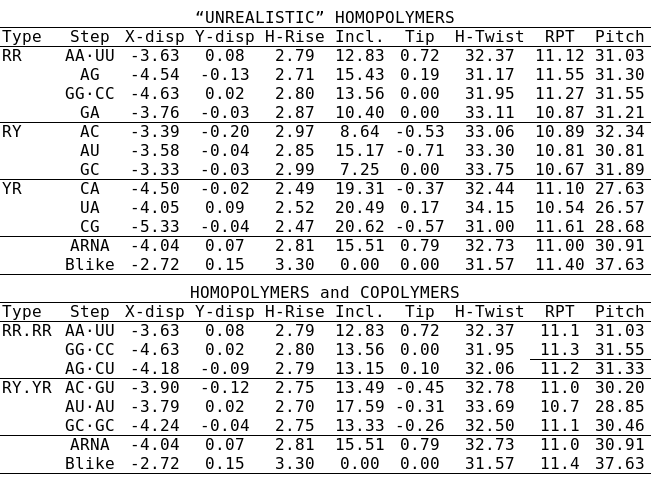
\includegraphics[angle=0, scale=0.66]{Chapter4/helicalprop.png}
\caption{Helical parameter values  for the homopolymers and copolymers
  built using  3DNA from the average  base-pair-step parameters values
  of  averaged  crystallographic data.  For  corresponding images  see
  Figure \ref{fig:homohetero}}
\label{fig:helicalprop}
\end{figure}


As  is the  case with  DNA, the  poly rA$\cdot$poly  rU chains  show a
smaller  persistence length  than  the poly  rG$\cdot$poly rC  chains,
although the difference is not as dramatic as that shown by Maroun and
Olson \cite{maroun1988a} for  DNA. That is, the difference  for DNA is
about $\sim$500  \AA, and  for RNA the  difference is  about $\sim$100
\AA.  The stiffer polyrG chains in this case reflects more symmetrical
energy surface  as is the case for  DNA, this can easily  be seen from
the corresponding energy surfaces available at our web-framework where
the energy  contour for the GG$\cdot$CC  step is circular  and the one
for AA$\cdot$UU base-pair step has the shape of an ellipse.

With 3DNA  we can build a  rigid block model  representation using the
average rest states from the  averaged crystallographic data to have a
fast representation  of what  this conformations look  like as  can be
seen in Figure \ref{fig:homohetero}.

\begin{figure}
\centering
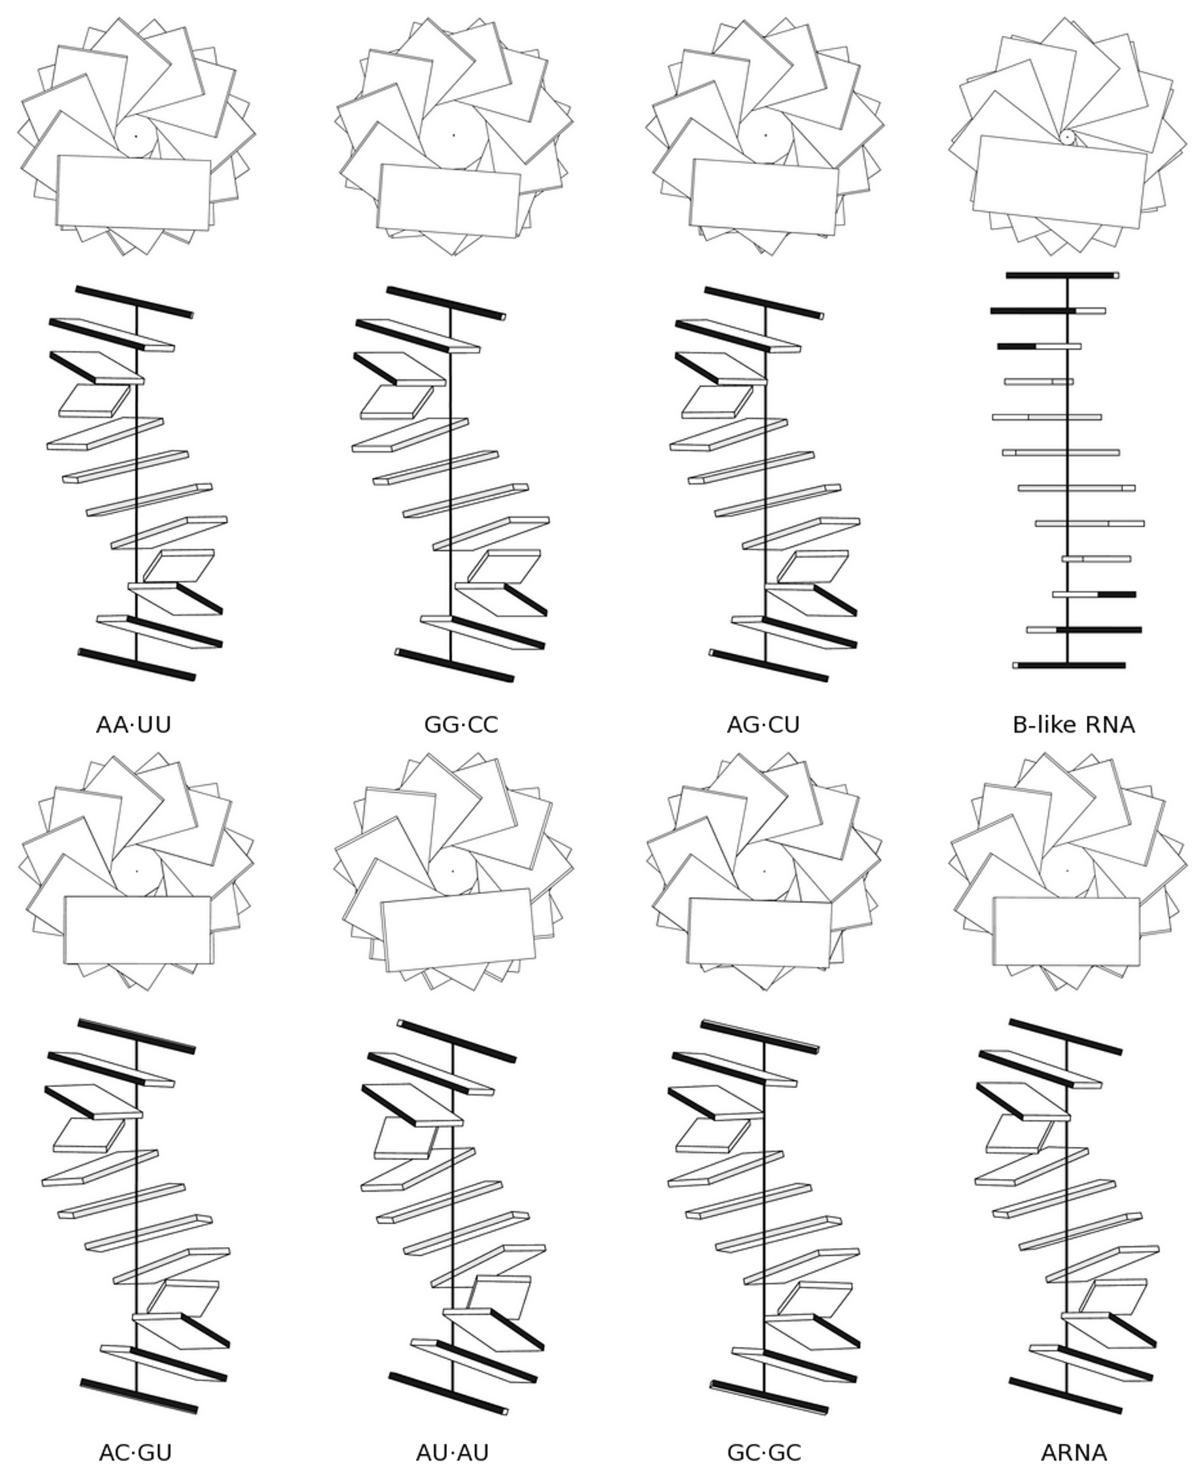
\includegraphics[angle=0, scale=3.0]{Chapter4/homohetero.png}
\caption{Calladine-Drew like block representation \cite{calladine1997}
  made from the rest states for  the ten unique base-pair steps in RNA
  from averaged crystallographic data. The structures were built using
  3DNA \cite{lu2003}.}
\label{fig:homohetero}
\end{figure}

For comparison  with sequence dependent properties of  DNA we computed
the persistence  length of RNA sequences of  1000 base-pair-steps made
up of repeats of the  unique base-pair steps, taking a million samples
with the Gaussian sampler and  assuming a naturally straight chain. As
can be seen in the results in Table \ref{tab:compare}, the persistence
length  is generally  larger than  the  obtained for  DNA (using  such
data).   The dependence reflects  the greater  stiffness of  the A-RNA
dimers  compared to the  more flexible  B-DNA conformation,  which RNA
cannot assume.

We also constructed a mixed  sequence RNA homopolymer with a 1:1 ratio
of A$\cdot$U to G$\cdot$C base-pairs, and 16 equally weighed base-pair
steps. The computed values  in Table \ref{tab:compare} are larger than
their  experimental counterparts,  as is  also  the case  for the  DNA
values.   We  therefore introduce  a  scaling  factor  to compute  the
persistence  lengths  (Table   \ref{tab:compare}).  To  obtain  values
according to those of Abels et  al. a $\zeta$ scaling value of 0.75 is
necessary to bring  the persistence length of the  random sequence RNA
to a value of 638 \AA.

\begin{table}  
\begin{center}
%\scalebox{0.7}{
\begin{tabular}{|c|c|c|c|}
\hline
Stack Type & Base-pair Step & $a$ (\AA) RNA & $a$ (\AA) DNA\\
\hline \hline
RR &  AA$\cdot$UU & 758      &  789   \\
   &  AG$\cdot$CU & 1116     &  919   \\
   &  GG$\cdot$CC & 1099     &  808   \\
   &  GA$\cdot$UC & 1115     &  785   \\
\hline
RY &  AC$\cdot$GU & 539      &  1245   \\
   &  AU$\cdot$AU & 818      &  490   \\
   &  GC$\cdot$GC & 1166     &  904   \\
\hline
YR &  CA$\cdot$UG & 536      &  779   \\
   &  UA$\cdot$UA & 820      &  435   \\
   &  CG$\cdot$CG & 1117     &  534   \\
\hline
   & Mixed Sequence  & 911   &        \\
   & Hagerman   & 700-800    &        \\
   & Abels et al.   & 622    &        \\ 
   & Abels et al.   & 638    &        \\
   & Ideal DNA    &          & 510    \\
   & $\zeta$ (scaling factor)  & 0.75 & 0.50 \\
\hline
\end{tabular}
%}
\caption{Persistence lengths for chains of 1000 base-pairs constructed
  from the ten unique base-pair steps. A scaling factor $\zeta$ is used to
  reproduce the experimentally obtained values of persistence length
  of a random sequence with equal weights of G$\cdot$C and A$\cdot$U
  base-pairs, and with an equally weighed composition of the sixteen
  unique base-pair steps.}
\label{tab:compare}
\end{center}
\end{table}

We also computed the  persistence length, at increasing chain lengths,
of      a      mixed       sequence      RNA      block      copolymer
(poly(AC)$_{\text{3}}$G$_{\text{5}}$)     as     seen    in     Figure
\ref{fig:curved}.     We   see   that,    in   contrast    to   Figure
\ref{fig:perVlen}, the chain-legth dependence of the mean extension of
the block copolymer seems to  be "damped".  The same sort of variation
in    the    persistence    length    occurs    in    DNA    sequences
\cite{maroun1988b}. A set of a hundred sampled configurations of a 150
bp long chain, obtained using  the Gaussian sampling technique and the
rebuild   feature  of   3DNA,   are  superimposed   using  the   first
base-pair-step   reference    frame   of   the    chains   in   Figure
\ref{fig:rnatree} and  viewable as a sequence of  independet images at
the                             web                            address
\url{http://rnasteps.rutgers.edu/rnadimer/media/img/movie.htm}.     The
series of  images reveal  the tendency for  the sequence to  curve and
therefore reduce the persistence length of RNA. The value of $\sim$340
\AA~ for the block copolymer is  much smaller than that for any of the
chains shown in Figure \ref{fig:perVlen}.

\begin{figure}
\centering
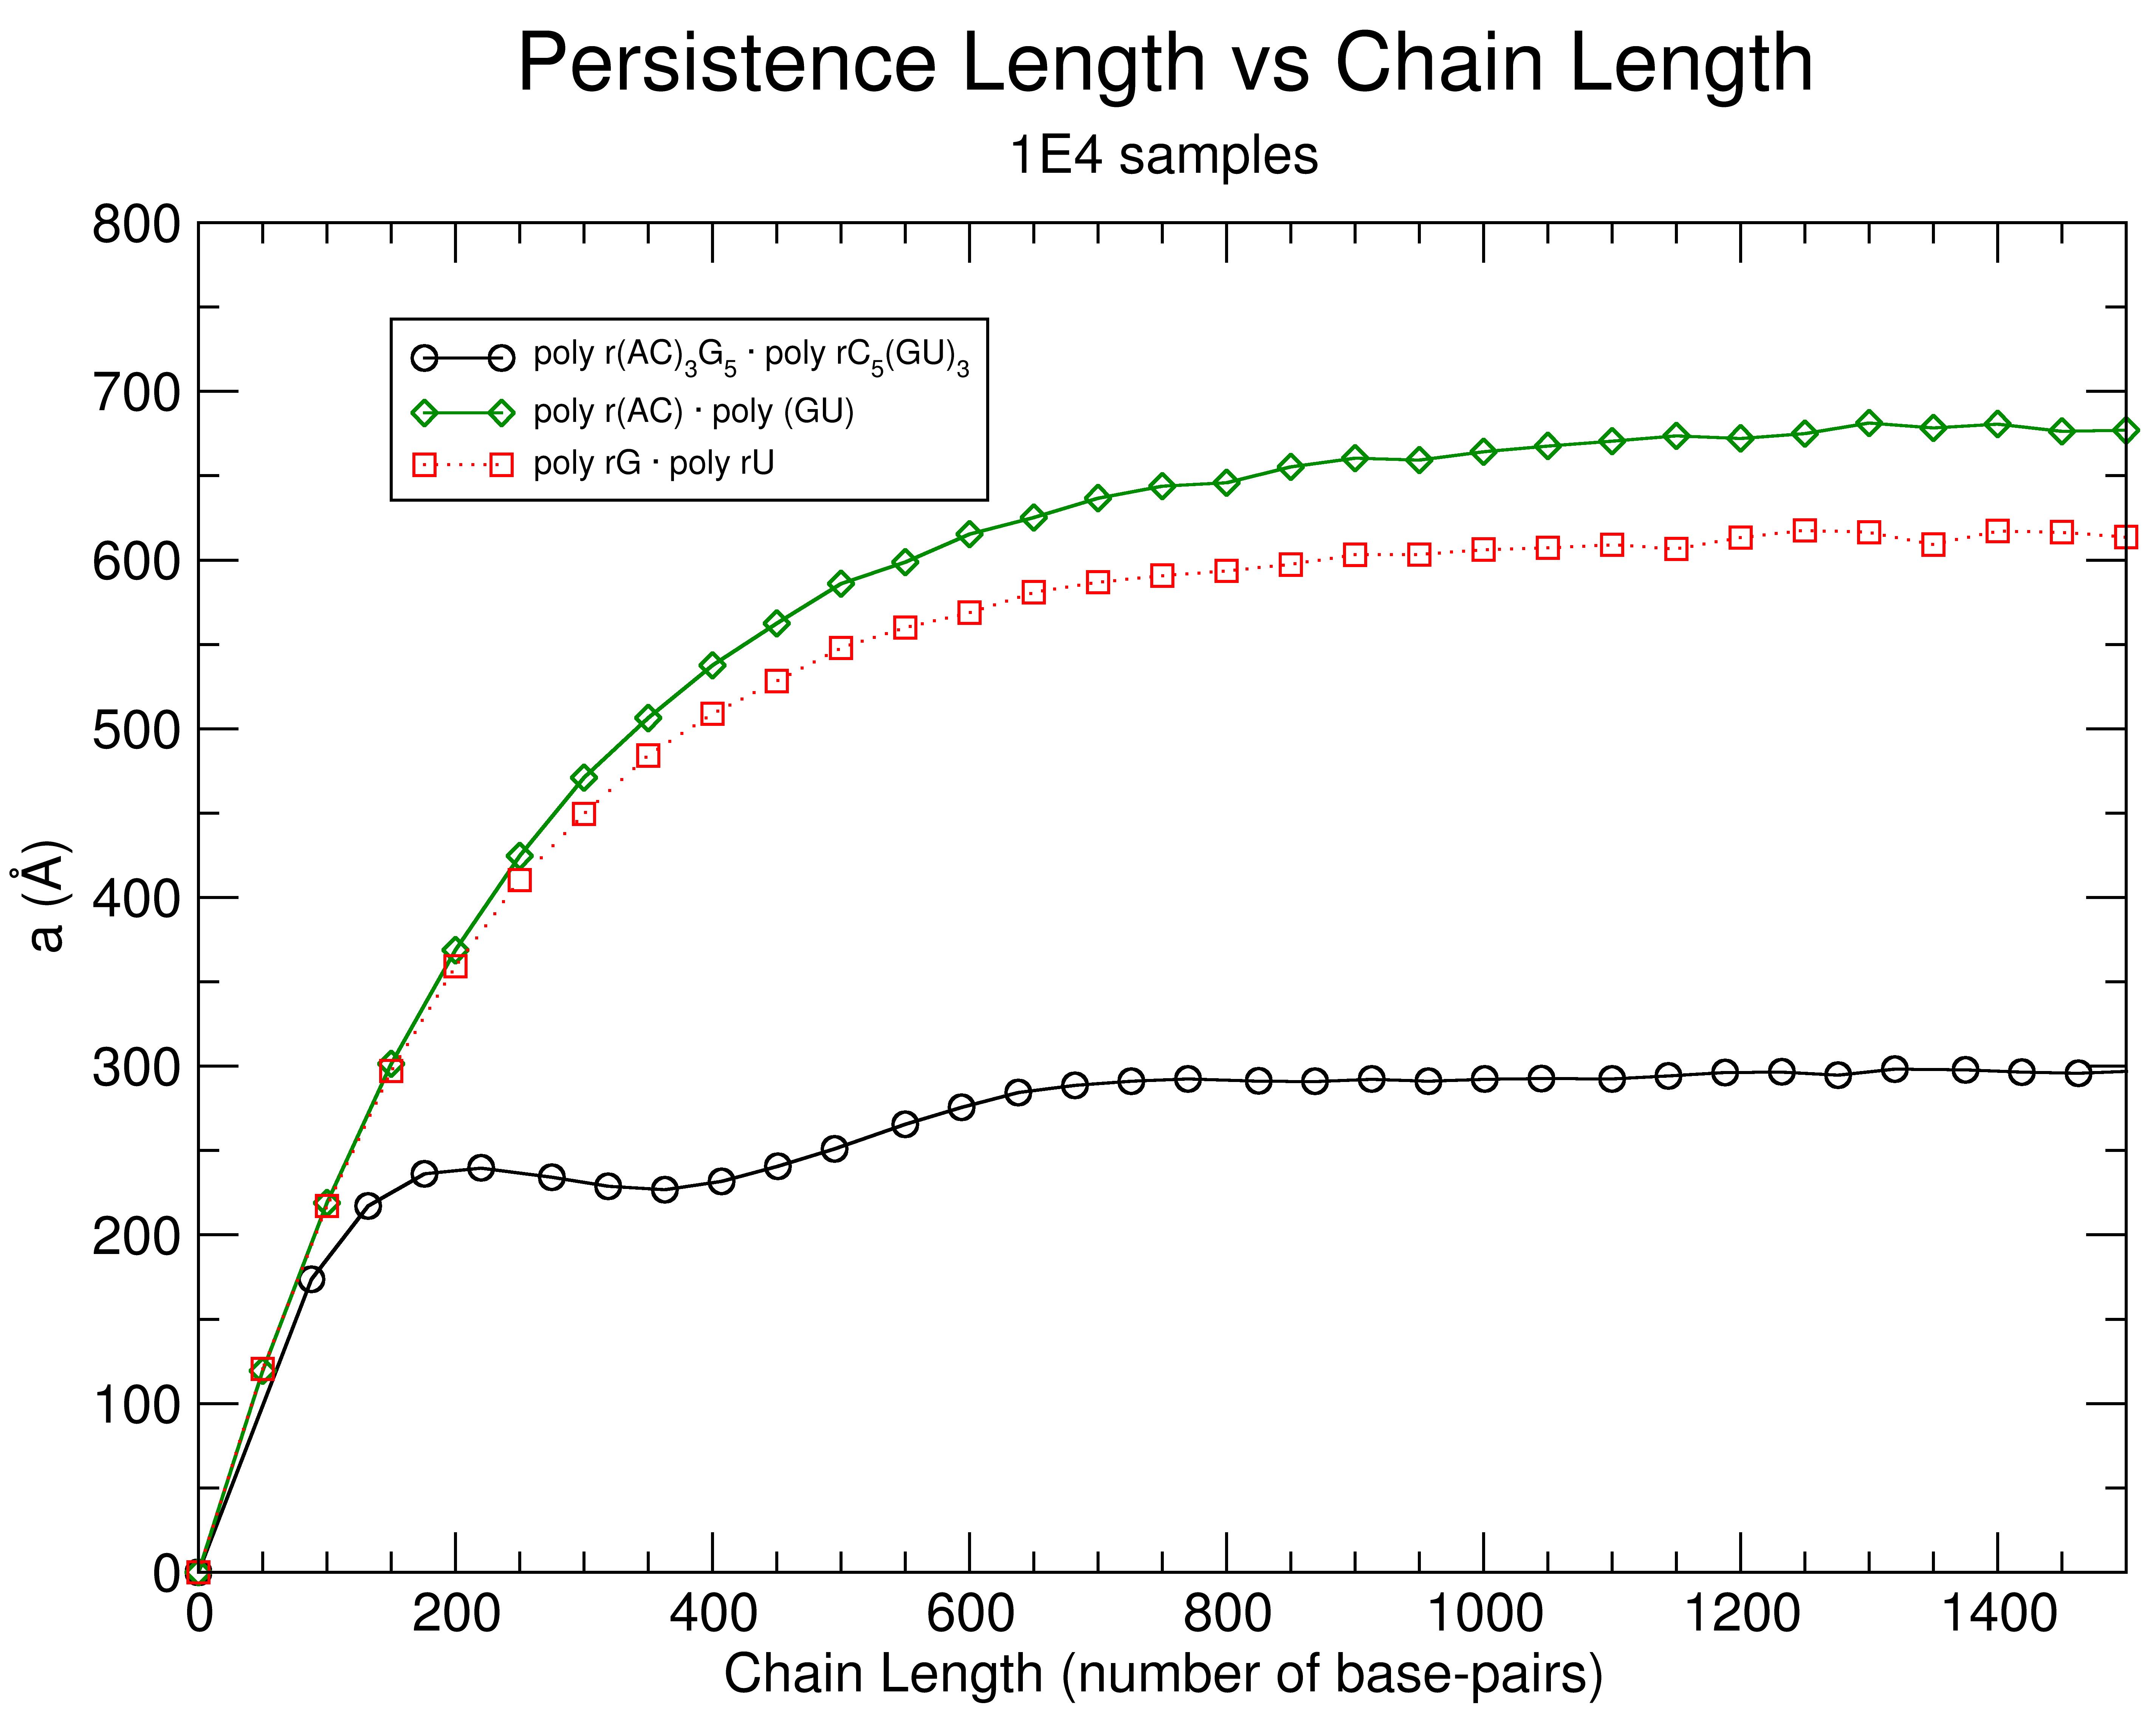
\includegraphics[angle=0, scale=0.6]{Chapter4/curved_and_steps.png}
\caption{Chain length  depence of the  persistence length for  the RNA
  block  copolymer   poly  r(AC)$_{\text{3}}$G$_{\text{5}}\cdot$  poly
  rC$_{\text{5}}$(GU)$_{\text{3}}$. Configuration samples obtained
  using    the   Gaussian    sampling   technique    of    Czapla   et
  al. \cite{czapla2006}. The curved  pattern is indicative of a curved
  or super helical configuration in RNA induced by sequence.}
\label{fig:curved}
\end{figure}

\begin{figure}
\centering
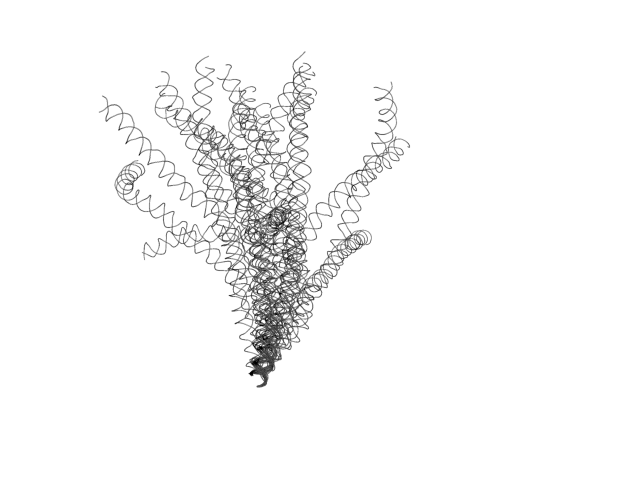
\includegraphics[angle=0, scale=2.0]{Chapter4/polyacacacggggg_all.png}
\caption{RNA   chains   of   the   150  bps   block   copolymer   poly
  r(AC)$_{\text{3}}$G$_{\text{5}}\cdot$                            poly
  rC$_{\text{5}}$(GU)$_{\text{3}}$ superimposed in the reference frame
  of the  first base-step.   Shown are a  100 snapshots of  the output
  produced  by  building  the  structures from  the  randomly  sampled
  step-parameters  obtained with  the Gaussian  sampling  technique of
  Czapla et al. \cite{czapla2006}.  Each chain is depicted by a ribbon
  linking sequential phosphorous  atoms, reconstructed using 3DNA from
  the base-step parameters at each dimer step.}
\label{fig:rnatree}
\end{figure}  






%\section{AMBER: Persistence Length of Base-Pair Step Patterns}
%I guess it needs some input here in order to work on latex compilation.



%CHAPTER OUTLINE

%- Methods Paper Results / Trends from counts
%  - Data culled.
%- Step Parameters. Conf Vols, RMSD
%- Equipotential Curves

%- Webserver
%  -table counts
%  -table force constants
%  -potential curves
%  -superimposed structures

%- Persistence Length RNA


% Technical pipeline details
%- Collection of base-pair steps data in helical regions.
%  - Yurong's bps database
%  - Yurong's python 3dnaparser
%  - scripts to change signs, assamble unique steps, and do stats.
%  - scripts to cull data
%  - scripts for deformation score
%  - reconstruction and RMSD calculation
%  - scripts for force-constant-matrices


\bibliography{biblio}

